\begin{figure}[H]
    \centering
    \begin{subfigure}[b]{0.22\textwidth}
        \centering
        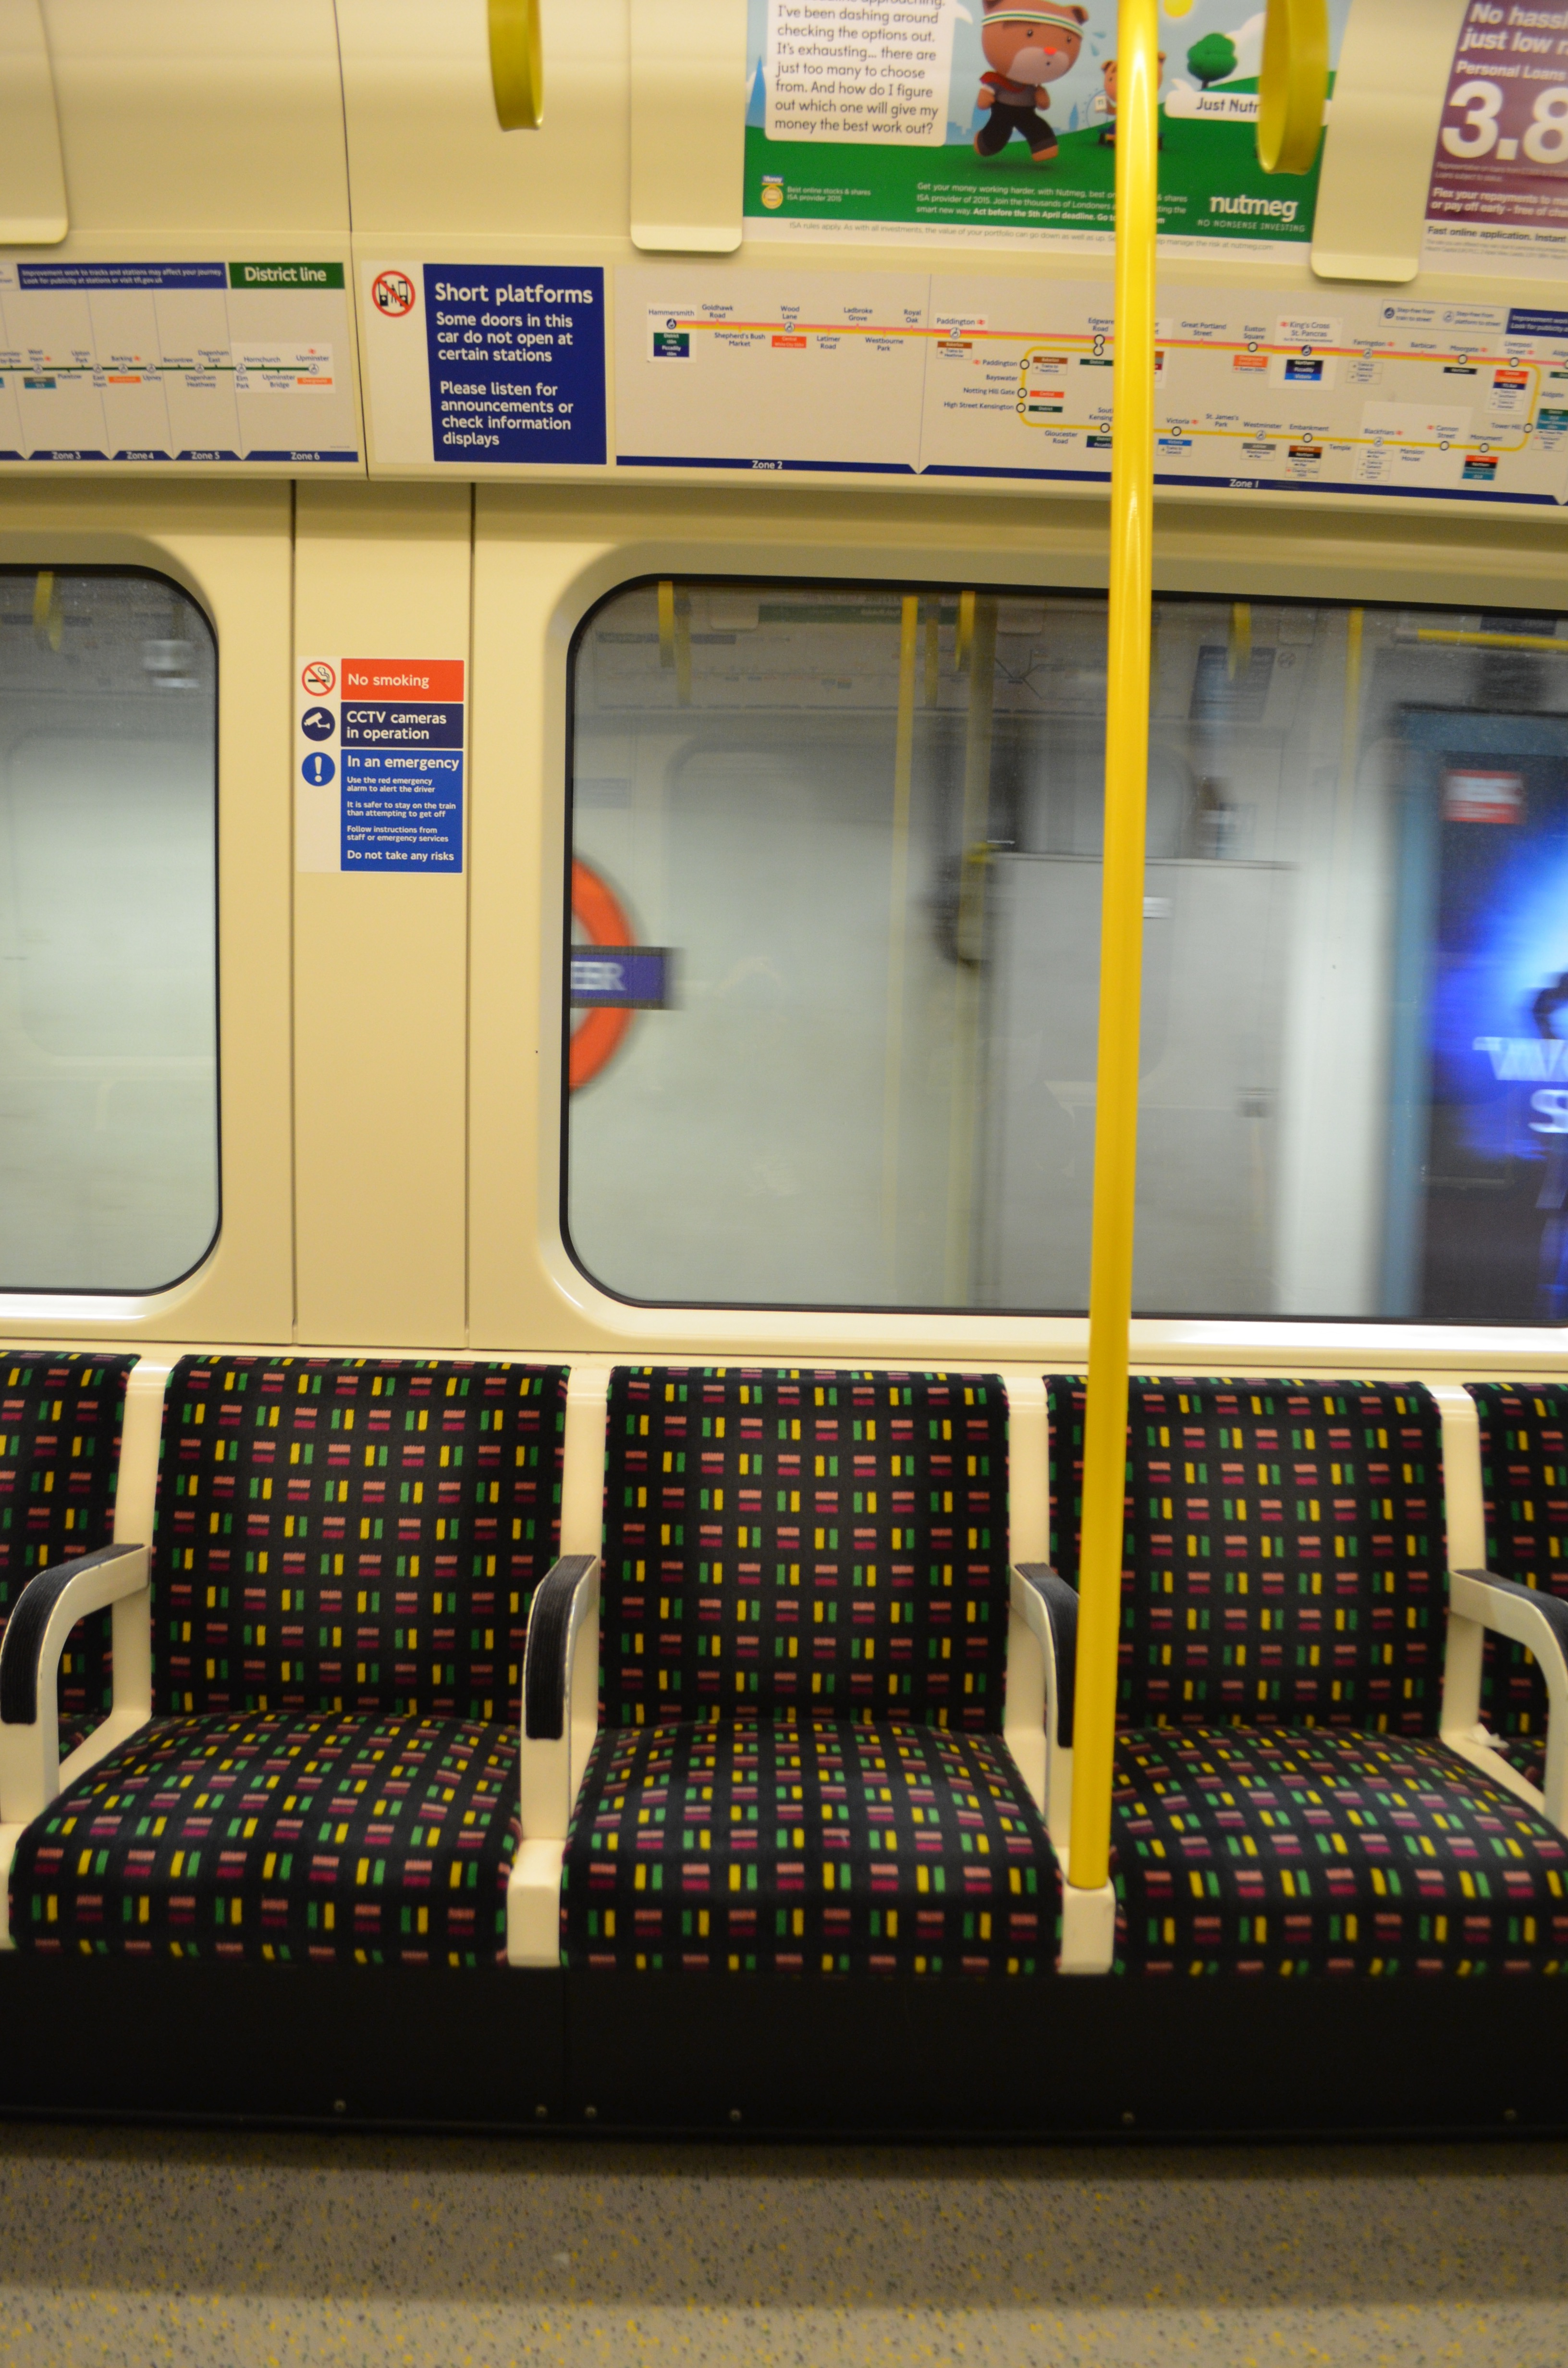
\includegraphics[width=\textwidth]{guidance-example-section/images/rathbone2017circle.jpg}
        \caption{Circle line \parencite{rathbone2017circle}}
        \label{fig:rathbone2017circle}
    \end{subfigure}
    \hfill
    \begin{subfigure}[b]{0.22\textwidth}
        \centering
        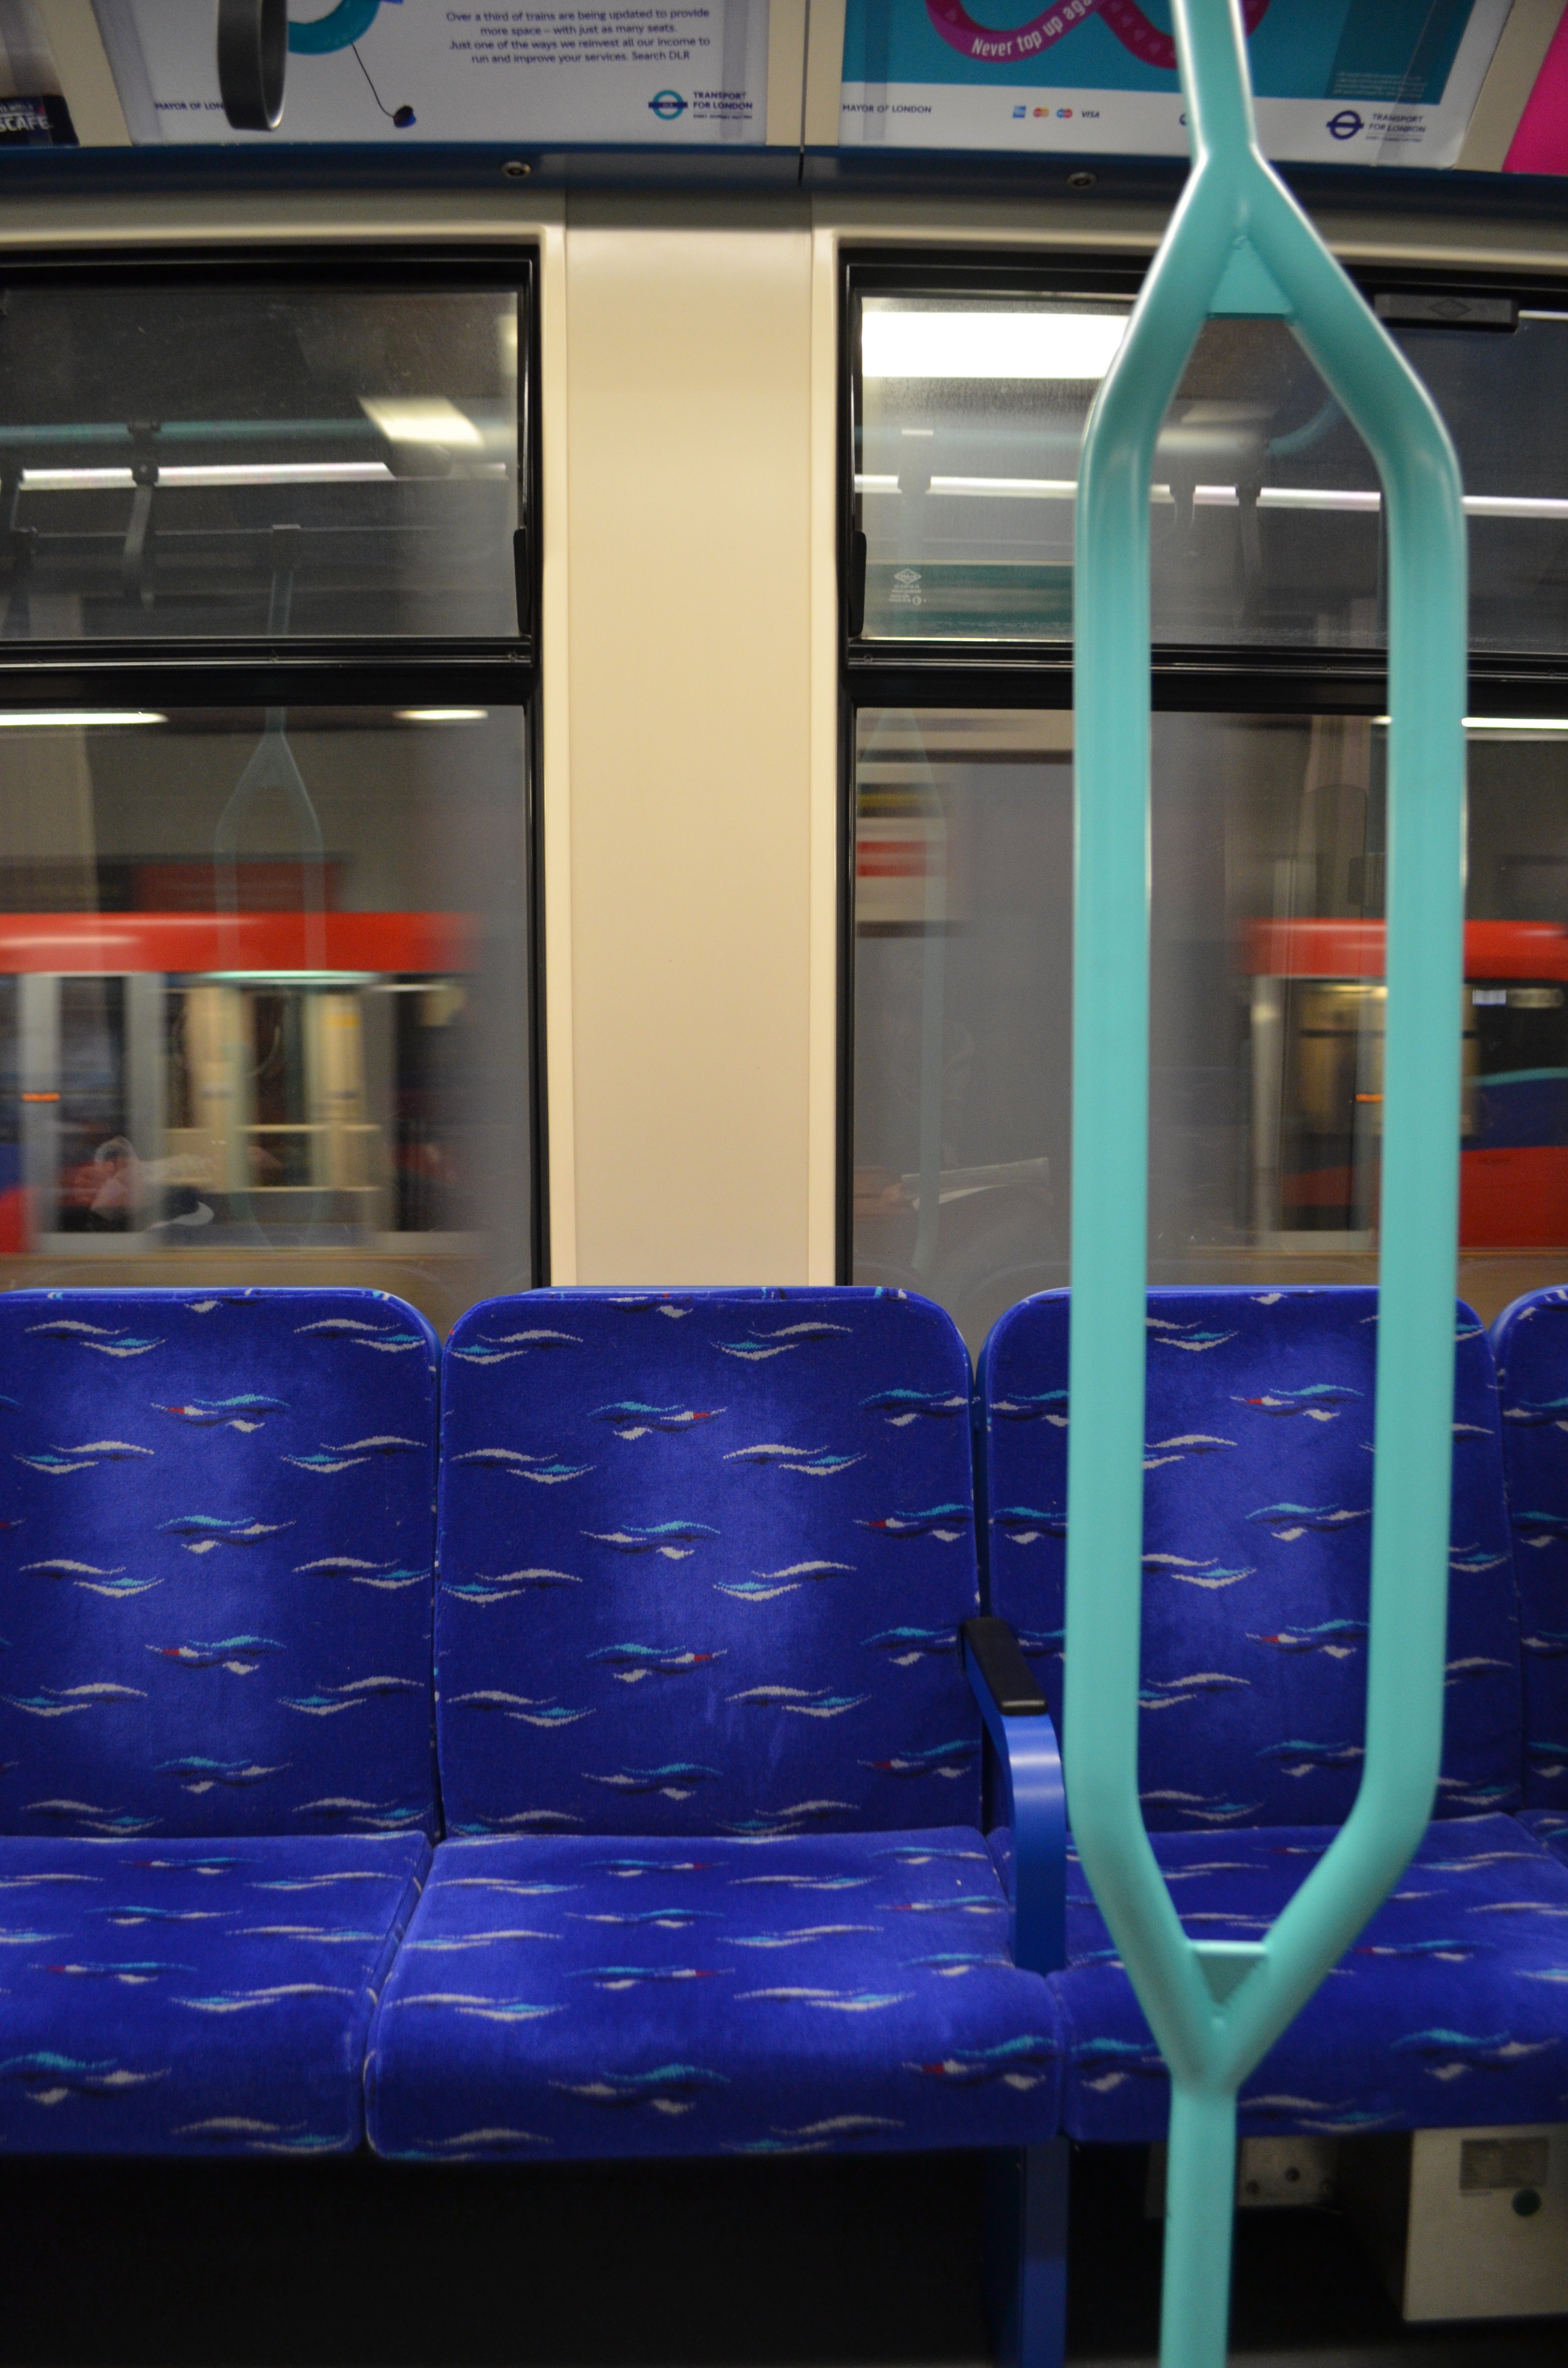
\includegraphics[width=\textwidth]{guidance-example-section/images/rathbone2017dlr.jpg}
        \caption{DLR \parencite{rathbone2017dlr}}
        \label{fig:rathbone2017dlr}
    \end{subfigure}
    \hfill
    \begin{subfigure}[b]{0.22\textwidth}
        \centering
        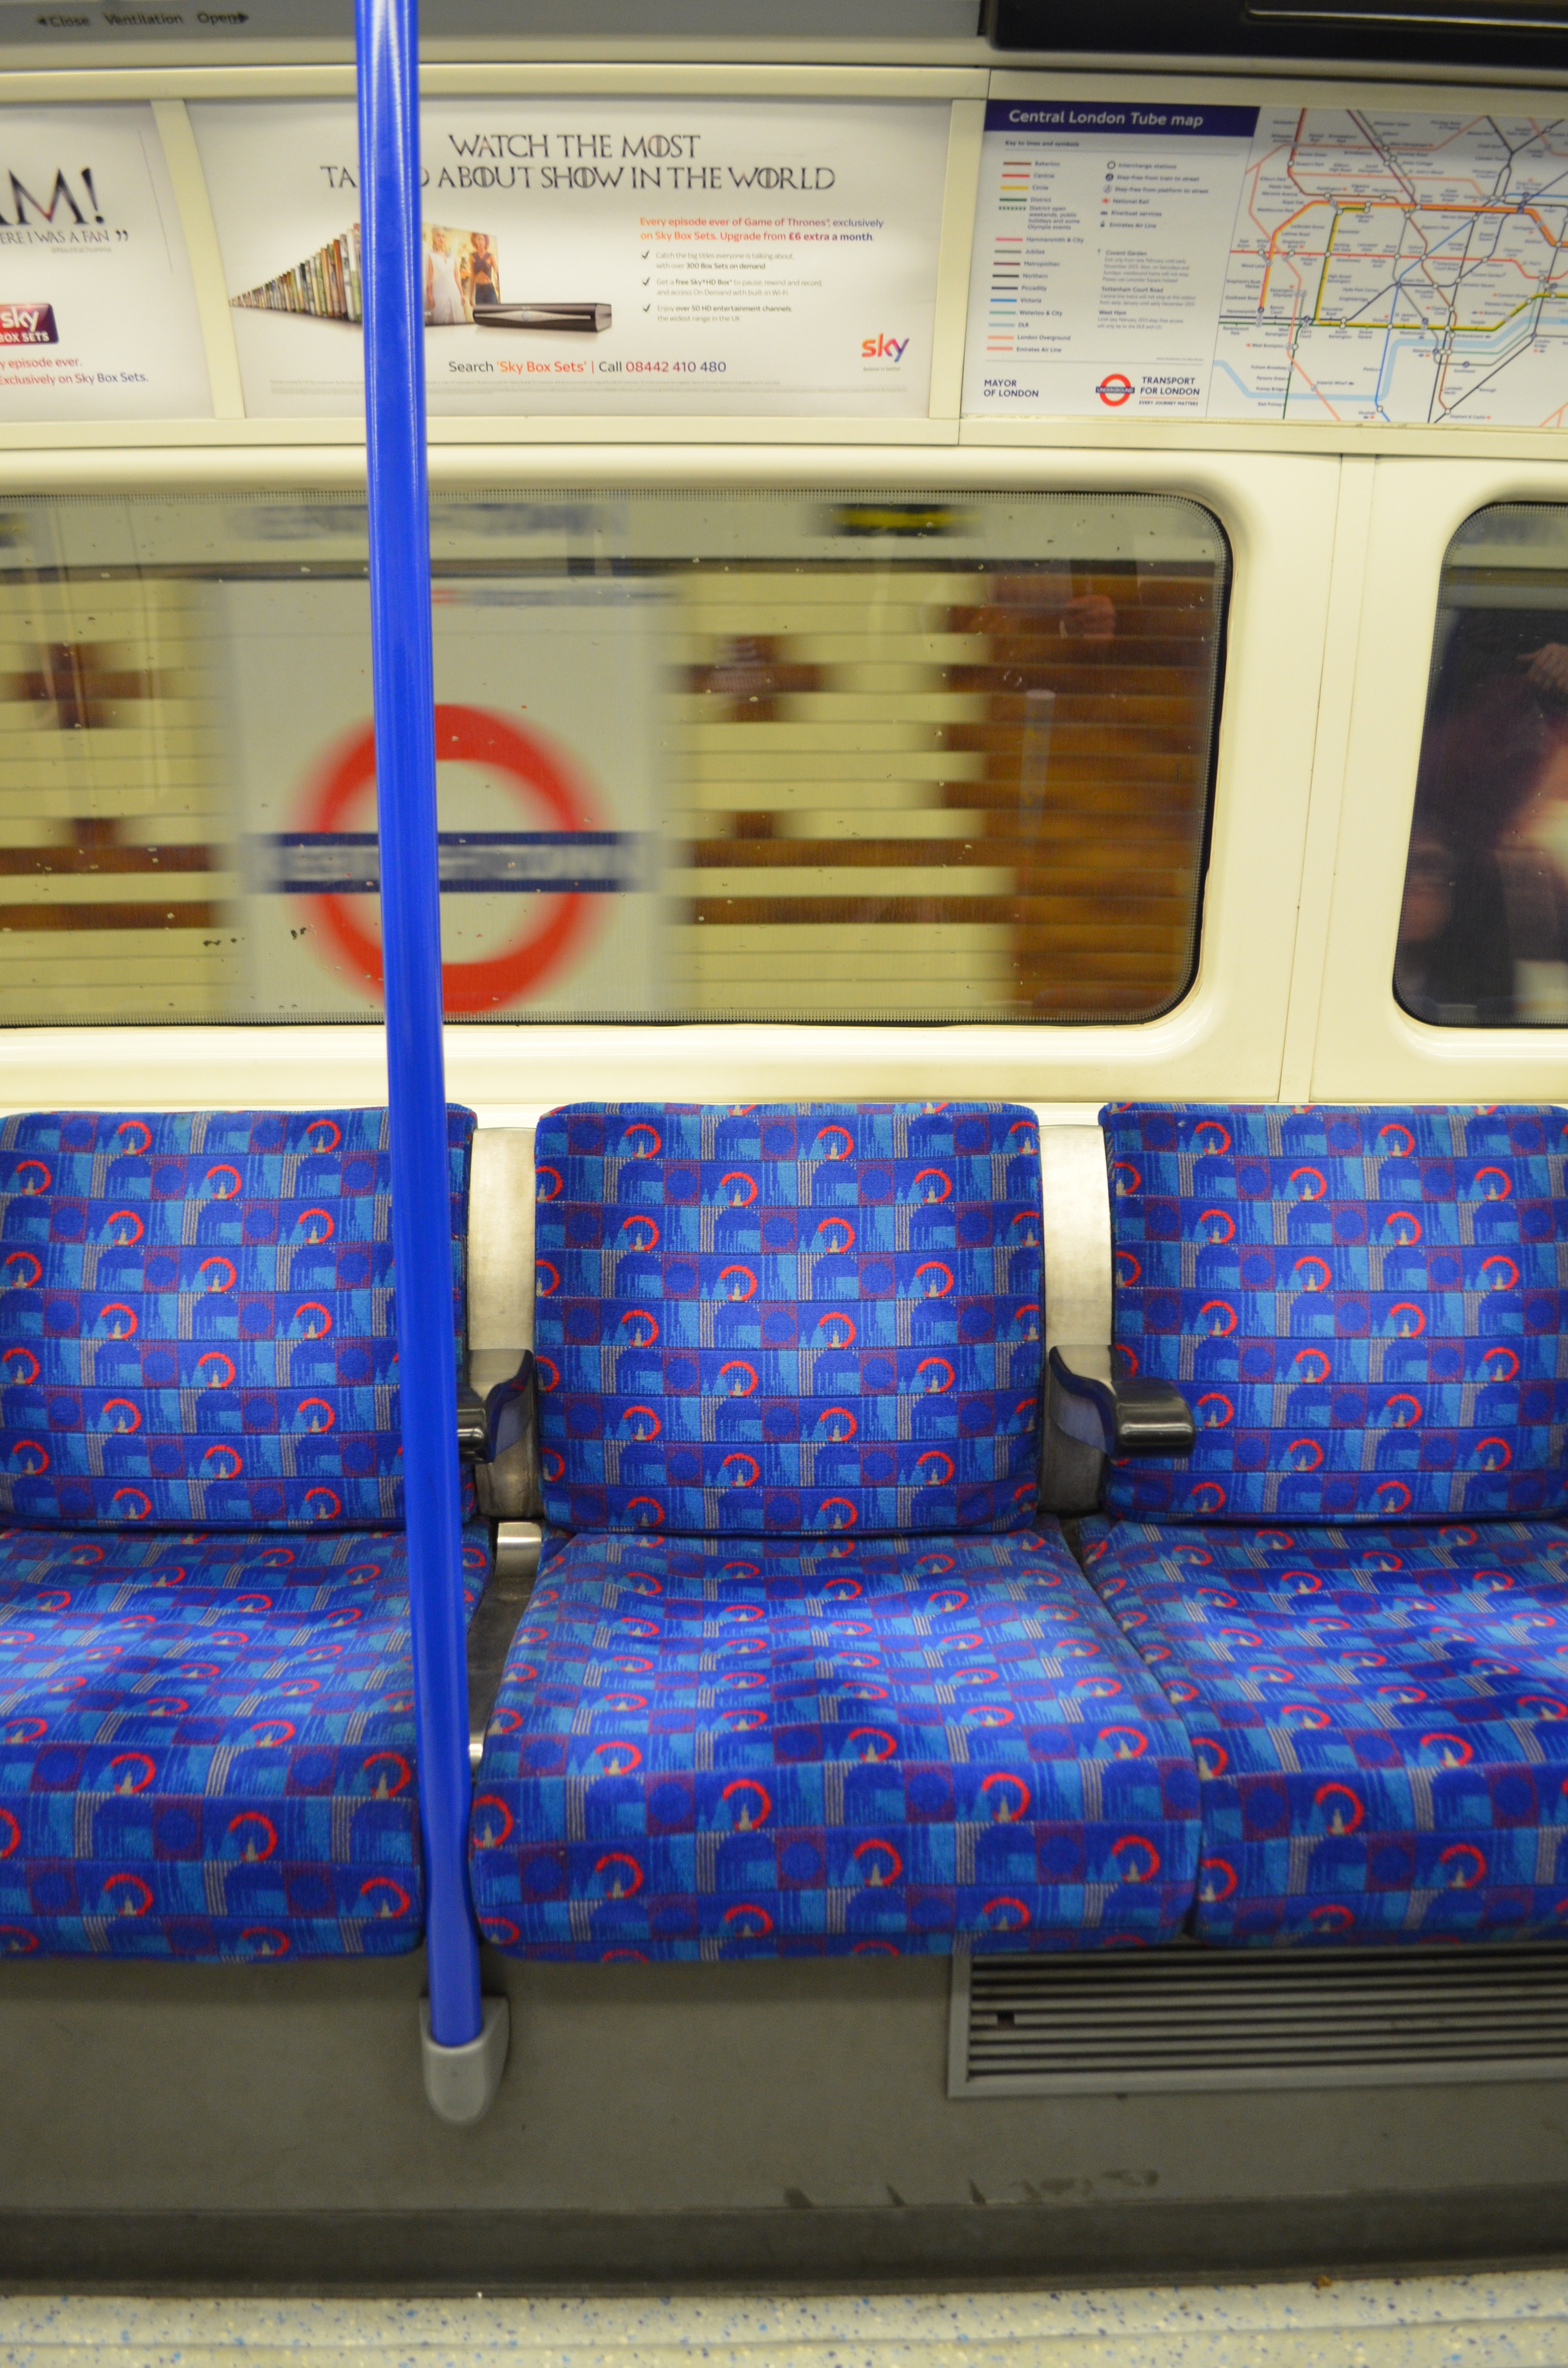
\includegraphics[width=\textwidth]{guidance-example-section/images/rathbone2017northern.jpg}
        \caption{Northern line \parencite{rathbone2017northern}}
        \label{fig:rathbone2017northern}
    \end{subfigure}
    \hfill
    \begin{subfigure}[b]{0.22\textwidth}
        \centering
        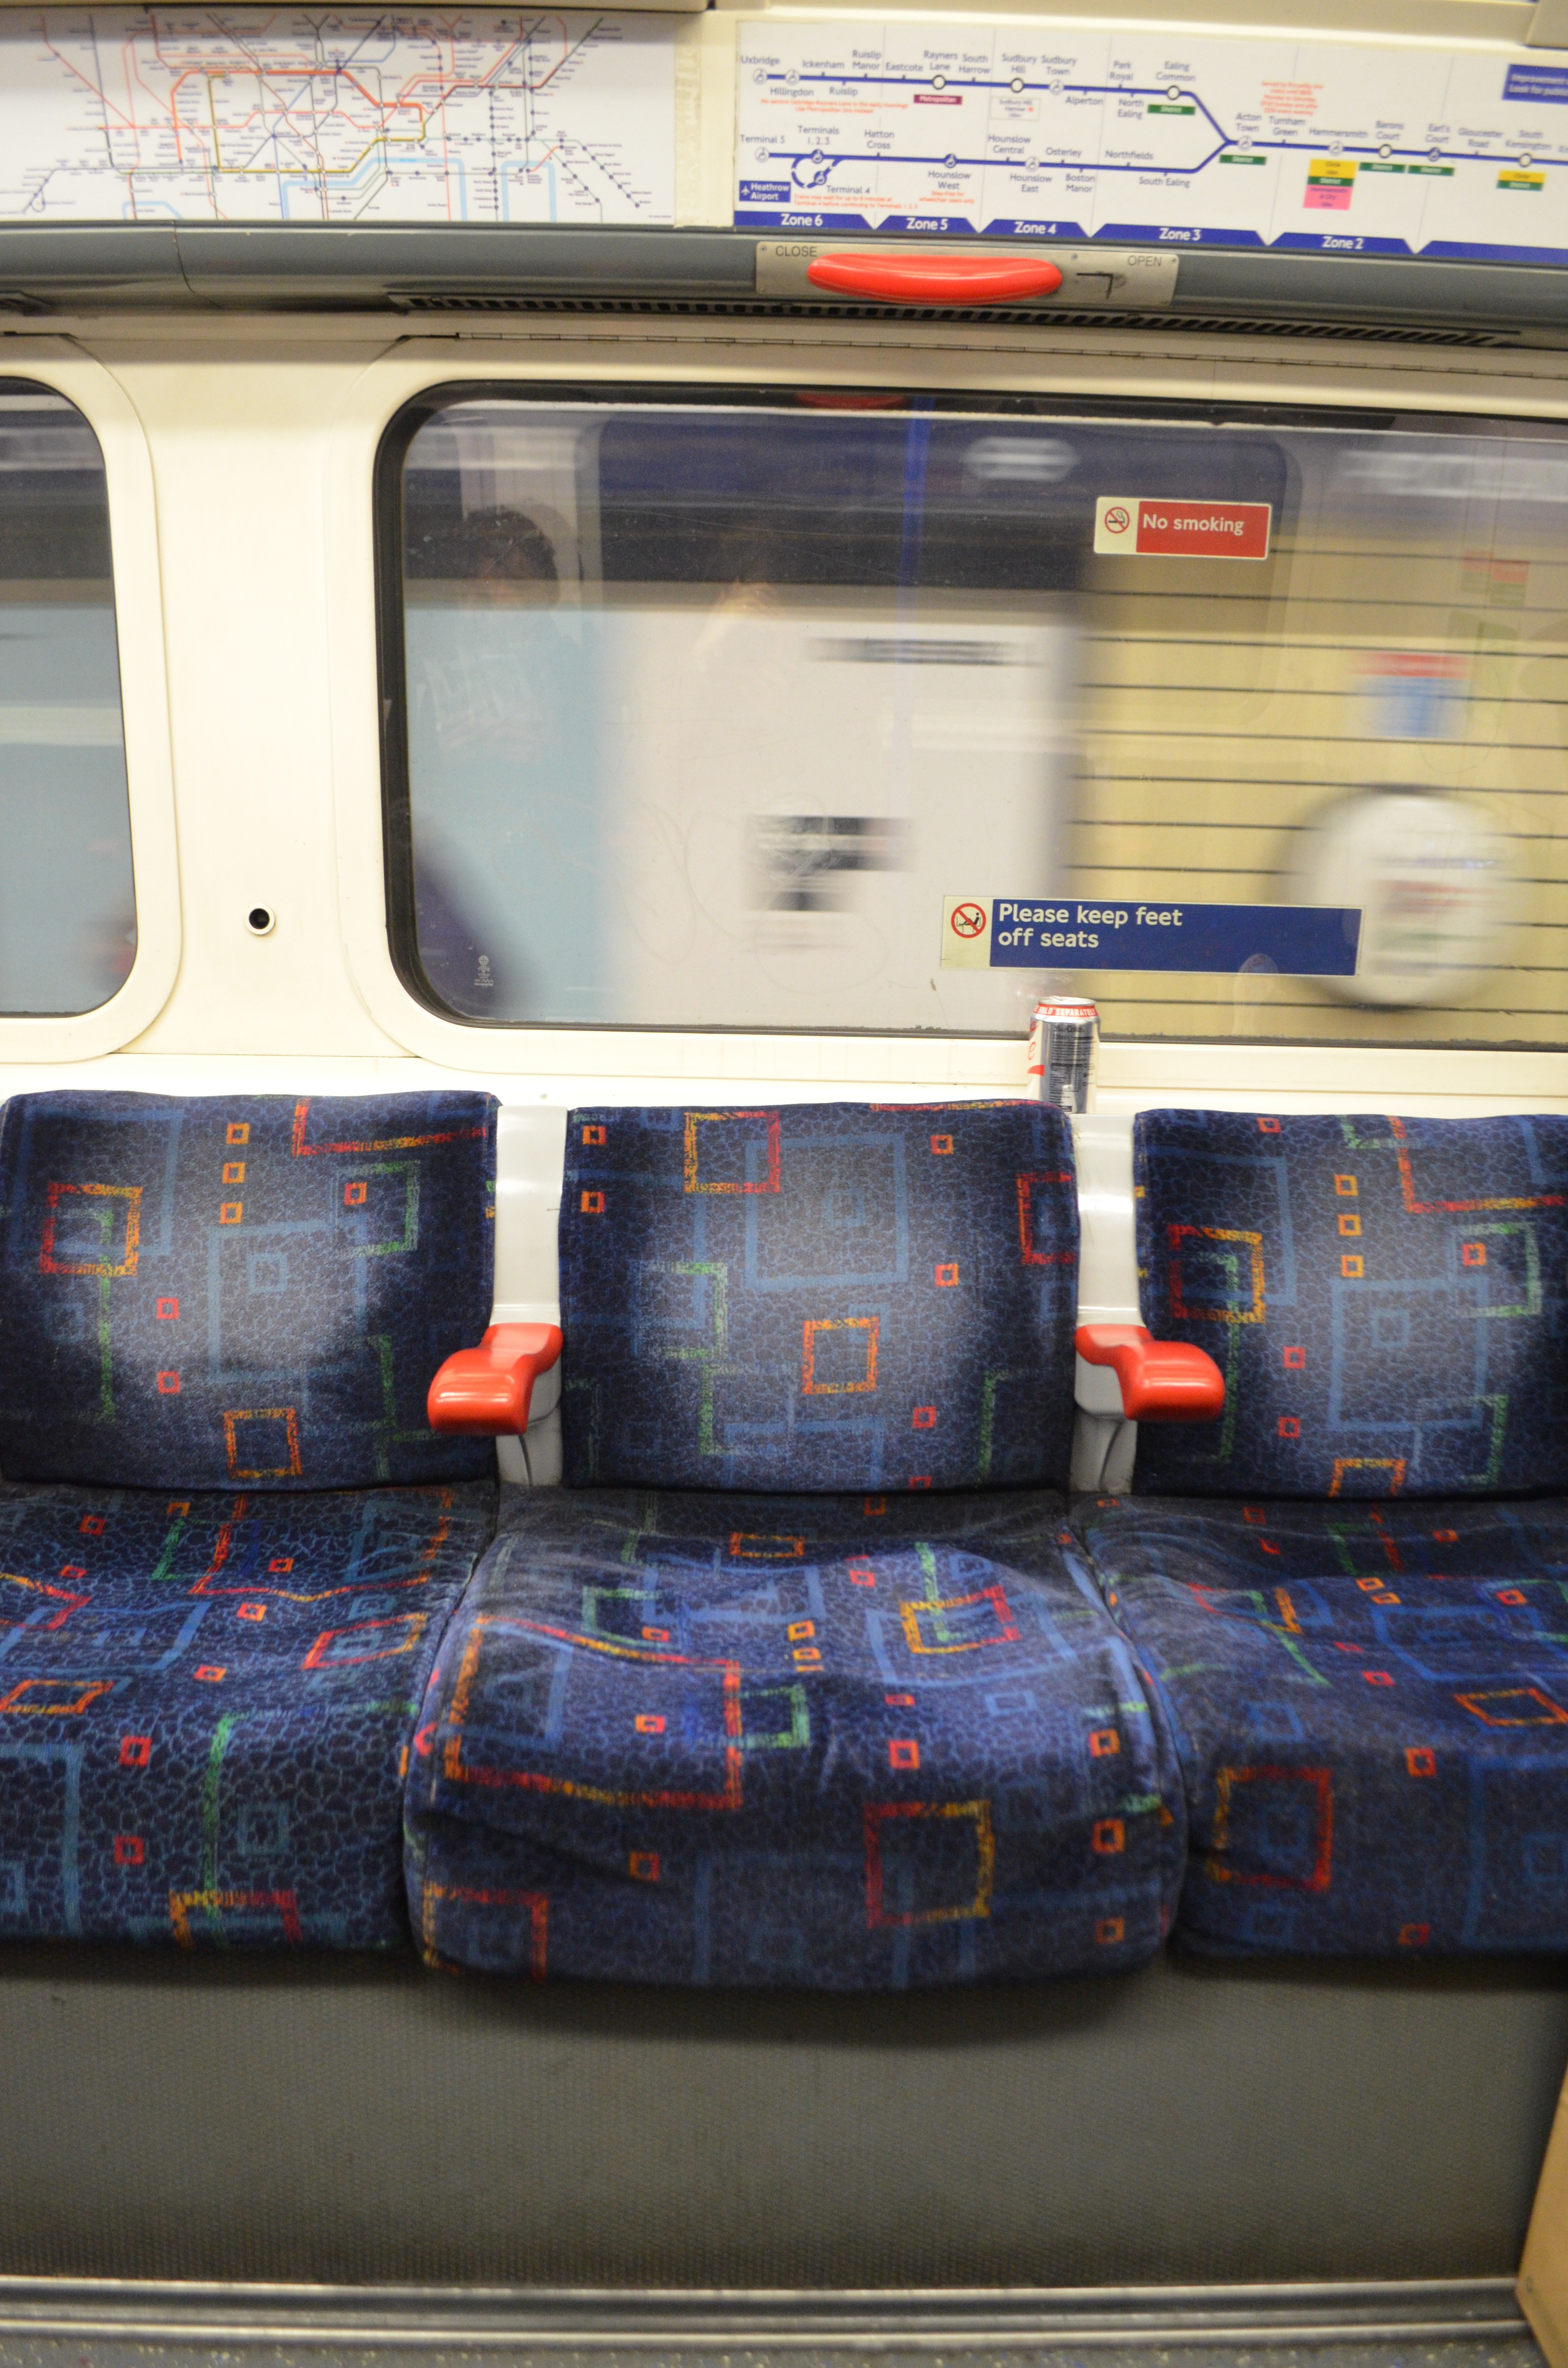
\includegraphics[width=\textwidth]{guidance-example-section/images/rathbone2017piccadilly.jpg}
        \caption{Piccadilly line \parencite{rathbone2017piccadilly}}
        \label{fig:rathbone2017piccadilly}
    \end{subfigure}
    \caption{4 examples of Transport for London seat cover patterns or "Moquettes". Courtesy of Loughborough University, accessed 10 October, 2024, \url{https://repository.lboro.ac.uk/projects/Transport_for_London_seat_cover_patterns/24400}}
    \label{fig:rathbone2017}
\end{figure}